% article document class appropriate for small (<100 pages) documents
\documentclass[draft, english, a4paper]{article}

% Packages provide additional functionality
%\usepackage{url}
\usepackage{fixme}
%\usepackage{lmodern}
\usepackage[final]{graphicx}%Force the graphics package to final, to force image inclusion
\graphicspath{{eps/}{images/}} %Set images/figures search path (relative to top latex file)
\usepackage[utf8]{inputenc}
\usepackage[left=3cm,top=4cm,right=3cm]{geometry}
\usepackage[dvips,
            colorlinks=false,
            pdfduplex=DuplexFlipLongEdge,
            pdfborder={0 0 0},
            pdftitle={Playing with LEGO},
            pdfauthor={Mikael Moghadam, Kenni Peter Isaksen, Morten S. Laursen,
                Robot Technology,
                SDU,
                Odense,
                Danmark},
            pdfsubject={Introduction to Artificial Intelligence},
            pdfkeywords={LEGO, Sokoban, line follow},
            plainpages=false,
            final]{hyperref}

\title{Playing with LEGO}
\author{Mikael Moghadam, Kenni Peter Isaksen, Morten S. Laursen}

\begin{document}

\maketitle % reads info from \title and \author above


% where BibTeX should read the bibliography records from and what
% style of bibliography it should generate
%\bibliographystyle{plain}
%\bibliography{}
\section{Introduction}
\newpage
\section{Architecture}
	\subsection{Division of responsibilities}
\section{Robot description}
        The prototype described in this section is to carry out the assignment as
        decided by the planner. In order to accomplish this task a robot 
        has been created. The robot is created using the LEGO NXT platform.  
	\subsection{Physical Construction} %Morten  
	    \label{robot:physicalContruction}
	    \fixme{Insert Robot picture here}
	    The robot is constructed using two motors which applies force to
	    each of their front wheels, this allows the robot to steer using skid steering.
	    As close as possible to the center of rotation during turns, three light
	    reflectance sensors is placed as illustrated in figure \ref{fig:lightSensorPlacement}
	    \begin{figure}[htp]
            \centering
    	    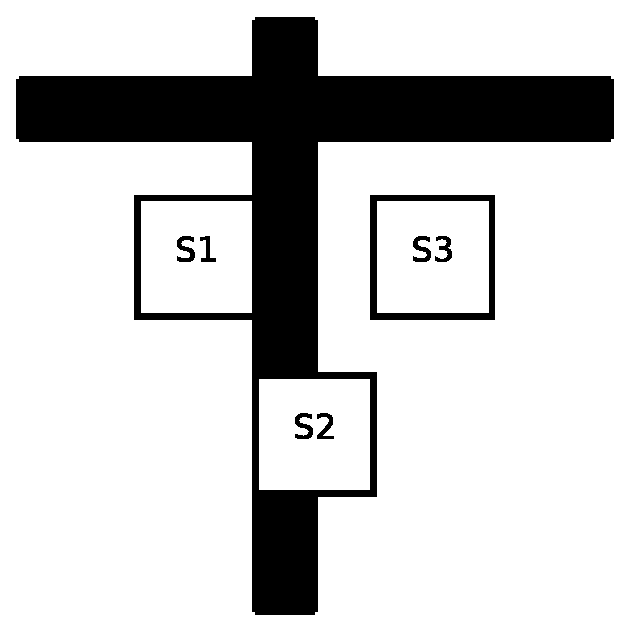
\includegraphics[scale=0.45]{lightSensorPlacement}
	        \caption{Illustration of light sensor placement, with the sensors mentioned S1-S3}\label{fig:lightSensorPlacement}
        \end{figure}
	    This allows the robot to detect either side of the line and thereby to
	    follow it, furthermore it allows the robot to detect when crossing a 
	    line.
	      
	\subsection{Robot architecture}
	    The Software architecture for the robot is created to give an abstraction
	    of each layer with as little complexity as possible. The architecture
	    is best illustrated by the block diagram illustrated in figure \ref{fig:robotBlockDiagram}.
	    \begin{figure}[htp]
            \centering
    	    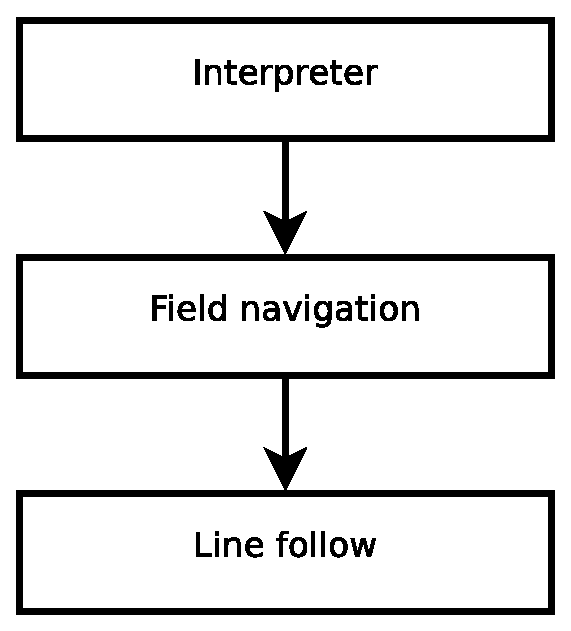
\includegraphics[scale=0.45]{robotBlockdiagram}
	        \caption{Block diagram of LEGO robot}\label{fig:robotBlockDiagram}
        \end{figure}
		%General introduction
		%block diagram
		\subsubsection{Interpreter} %Morten
		    The interpreter has to receive and interpret data from the routeplanner
		    and carry out that route using the field navigation block.\\
		    \\
		    The flow chart for the interpreter can therefore be described in the
		    following way
		    \begin{enumerate}
		    \item Receive/fetch command from routeplanner
		    \item perform command using field navigation
		    \item if more commands in cue goto 1, else exit
		    \end{enumerate}
		    Currently two options is under consideration for the interface between
		    the interpreter and the routeplanner, one is a simple file composed
		    of direction commands as delivered with the Sokoban example game.
		    The other option is to stream the commands using bluetooth, it is
		    anticipated that this would allow for easier debugging, and because
		    of existing libraries for bluetooth it should not cause much if any overhead.\\
		    \\
		    \fixme{For discussion: Should the interpreter or the routeplanner be responsible of
		    tomato can attack directions?}
%			What is the responsibility of this block
%			Block interface
%			Block design / bird perspective flow chart 
%			Block test
		\subsubsection{Field navigation} %Morten
		    The field navigation should navigate between field intersections
		    as illustrated on figure \ref{fig:robotFieldNavigation}.
		    This task should be accomplished using the line following block\\
		    \begin{figure}[htp]
                \centering
    	        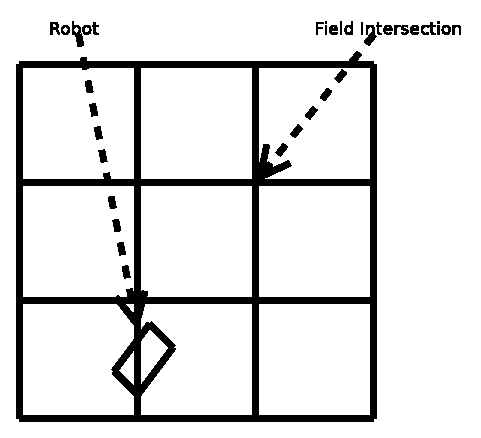
\includegraphics[scale=0.45]{robotFieldNavigation}
	            \caption{Illustration of playing field}\label{fig:robotFieldNavigation}
            \end{figure}
		    \\
		    As described in section \ref{robot:physicalContruction} the light
		    sensors is placed so that when following lines, only one sensor should
		    be active at a time, however when crossing a line both the left and the
		    right sensor should become active. This allows the robot to detect
		    crossing lines.\\
		    \\
		    When crossing a line the robot should first back up, so that the sensors
		    is placed over the crossing line, then rotate in the commanded direction
		    until a new line activates both sensors, then move one field
		    forward.
		    \fixme{Another option here is using the encoders
		    in reality we might test both and see which one performs best}
%			What is the responsibility of this block
%			Block interface
%			Block design / bird perspective flow chart 
%			Block test
		\subsubsection{Line follow} %Morten
		    The line following block has the responsibility of keeping the robot
		    constantly on the line using the sensors to allow for precise navigation.\\
		    \\
		    On figure \ref{fig:sensor_measurements} a plot of what the sensors
		    measures when driving on a line has been created. It is clear when
		    looking at the plot that the signal does not contain a lot of higher
		    frequency components and will therefore not gain much from being filtered,
		    except less phasemargin in the control system. These data was measured
		    doing a evaluation of a proportional feedback control system.
		    \\
		    \begin{figure}[htp]
                \centering
    	        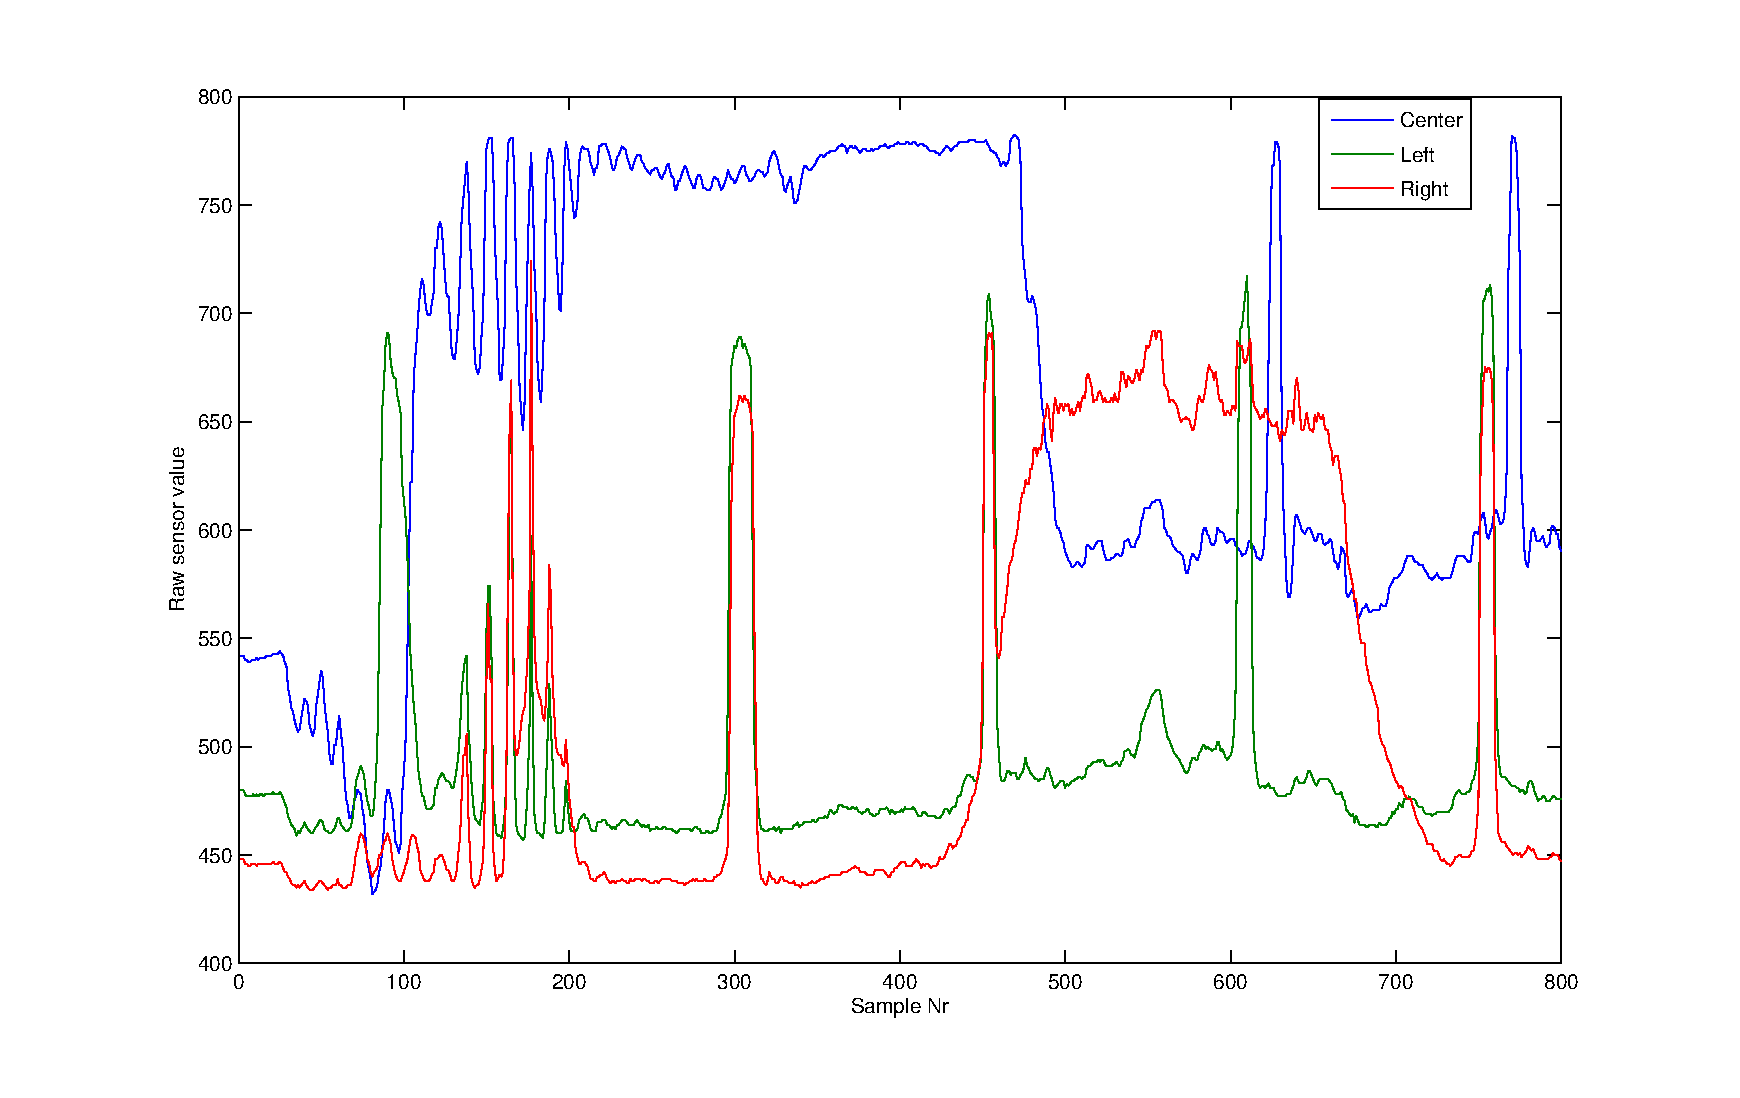
\includegraphics[scale=0.45]{sensor_measurements}
	            \caption{Raw samples of sensor measurements}\label{fig:sensor_measurements}
            \end{figure}
            \\
            \paragraph{Statemachine based}
            For making the control loop two different implementations has been
            tested, one using a simple state machine based solution, where the
            state machine tries to assess the position of the line as either left of the
            vehicle, centered below the vehicle or right of the vehicle and from
            this assessment tries to correct.\\
            \\
            \paragraph{PD-feedback based}
            Another option which has been tested is making a simple PD control loop
            using the light sensors, as the sensors are not entirely binary,
            but has a slight transition as more and more of the sensed area becomes
            line, it increases, a correction based on these small increases can 
            be seen as the oscillation between sample 100 - 200 on figure \ref{fig:sensor_measurements}
            Whereas the state machine based approach does not start correcting before reaching a threshold value.\\
            \\
            Having implemented both solutions on the vehicle the control loop based
            solution was chosen as it had the best performance.
		    %More detailed problem description with sensor position drawing
		    %measurement data examples.
		    %From there show proposed solutions
		    %Explain which one was chosen for which reasons, show flow diagrams
		    %of these two algorithms 
		    %Show incoming and output data from this block and the module test
%		    What is the responsibility of this block
%			Block interface
%			Block design / bird perspective flow chart 
%			Block test
	\subsection{Conclusion} %Morten
	    \fixme{Let us write this when the vehicle is done}
\section{Planner description}
	\subsection{Problem discussion, in the Sokoban domain} %Mikael
	\subsection{Discussion of path finding algorithms} %Mikael
		\subsubsection{Selection of algorithm}
	\subsection{Map representation} %Mikael
	\subsection{Algorithm design}
	\subsection{Performance evaluation}
	\subsection{conclusion}
\section{Conclusion}
\section{Discussion}
\appendix
\end{document}

